\chapter{Point Cloud Rendering}

As stated in~\citet{PointRendering}, using point primitives for rendering has been driven
by two main reasons. Over the years,
there was a dramatic increase in the polygonal complexity of models being rendered, leading to
the overhead of managing and processing extensive mesh connectivity information.
Further, modern 3D scanners (LiDAR, stereo camera setup) or photogrammetry methods (SfM) produce
both geometry and appearance of complex, real-world objects in the form of a point cloud. Points in a point cloud
play the role of (discrete) building blocks for 3D scenes, similar to how pixels are the digital ones for images.

Points are the simplest graphic primitive, generalizing pixels towards irregular samples of
geometry and appearance. They differ from triangles typically used in computer graphics
by carrying all attributes needed for processing and rendering with themselves the same way
as pixels do. That results in transformation of rendering pipeline, the terms vertex and fragment coincide in
one entity. Even though the presence of just one such entity may lead to simpler graphical pipelines,
it is not without issues~\citep{ComputeShaderRendering}.

1) Straightforward points projection leaves empty spaces in the image that need to be filled
for close-up views as it may lead to problems with occlusions and visibility or depth perception---with
less dense sampling, a render can end up with just many points scattered across
the background with no notion of what is closer and farther. Thus, point clouds typically
require a denser sampling compared to triangle meshes. 2) Points do not possess any topology or
connectivity information. This fact is an advantage and disadvantage at the same time, compared to
meshed that contain this type of information, but only as a result of 3D reconstruction
algorithms with point clouds being an input that typically still require some prior assumptions on topology
and sampling. It is, for instance, possible to stream and render point clouds progressively, and
change of topology (e.g., by filtering) is more straightforward than for meshes where one needs to recompute
connectivity information~\citep{PointRendering}. On the other hand, effective point processing typically needs
elaborate data structures, including KD-trees~\citep{KDTree} or spatial hashing~\citep{SpatialHashing}.

Over the years, many approaches have been devised for processing point primitives and tackling the
issues presented in the preceding paragraphs. In the thesis, we take advantage of having point clouds-based
datasets. We found out that for large indoor areas, it may be tricky to come up with sufficiently good
mesh that can be further used for the localization verification step rendering, as it can be seen
in~\cref{fig:mesh_artwin_render}. Proceeding with point cloud-based rendering techniques,
we work with three of them; please see the description below.

\begin{figure}
    \centering
    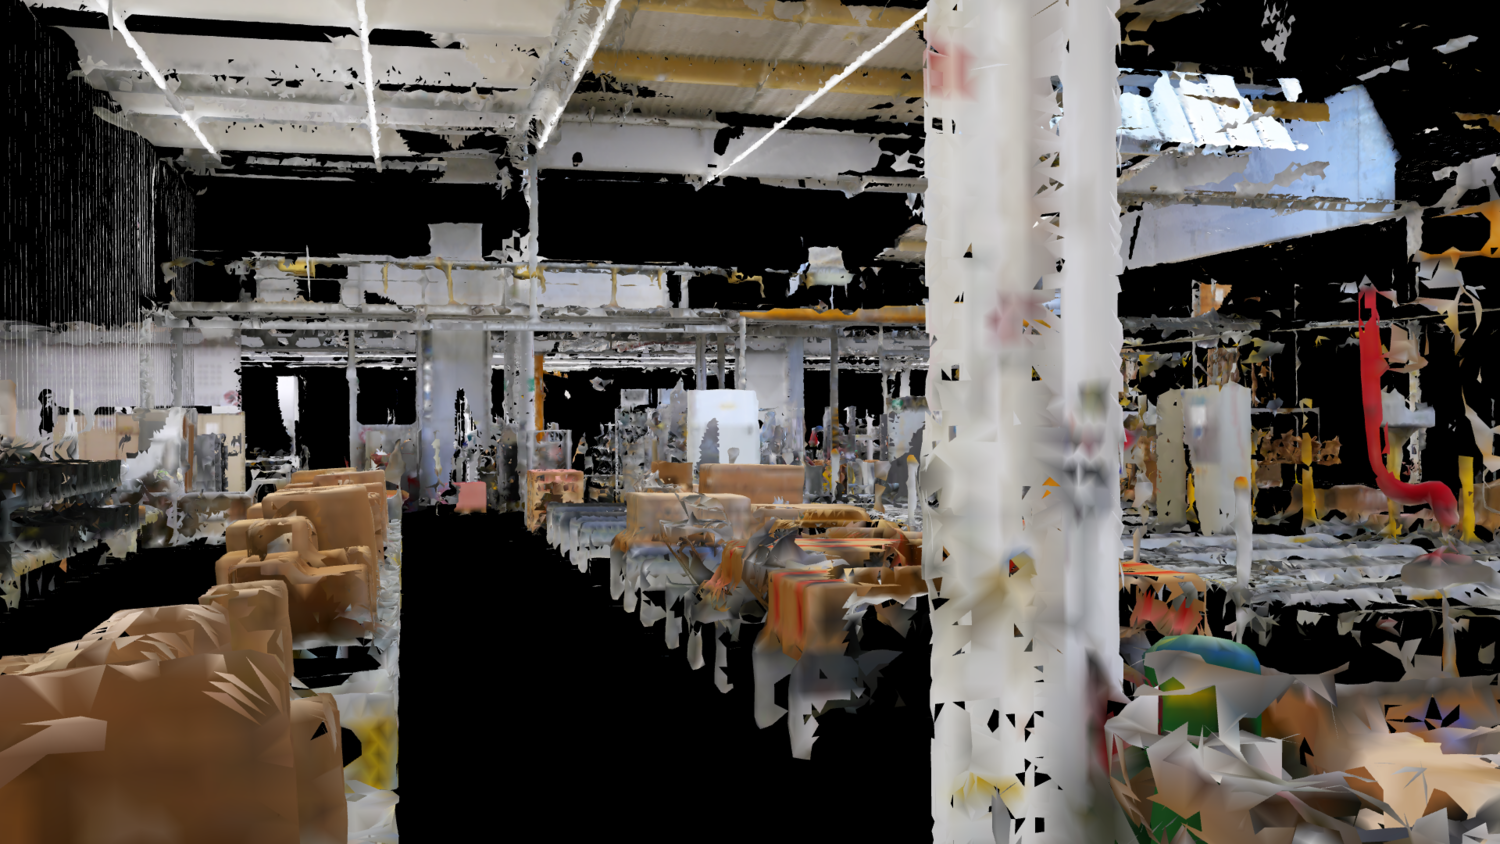
\includegraphics[width=.9\linewidth]{../graphics/0217_mesh_artwin_render.png}
    \caption{A render of one of the meshes created from the raw datasets' point cloud, camera pose is the same
    as for~\cref{fig:pyrender_artwin_render}. The mesh was created
    semi-manually, meaning that boxes, for instance, were meshed separately and then placed at the right
    place of the resulting mesh. We can see some disadvantages of using meshes in complex environments.
    Despite long processing time and laborious manual work, the result is not that compelling compared to renders
    using point primitives.}\label{fig:mesh_artwin_render}
\end{figure}

\section{Related Work}

\citet{SOTARendering} defined \emph{rendering} as transforming a scene definition, including some of the cameras,
lights, surface geometry, and material, into a simulated camera image. The process can be organized in two
ways~\citep{marschner2021fundamentals}. \emph{Object-order} rendering considers each object; for such,
all the pixels it influences are found and updated. In \emph{image-order} rendering, the loop
goes the other way round, each pixel is considered, and for such, all the objects that influence it are found, and
the pixel value is computed. From these two approaches, image-order rendering is simpler to implement and more capable in the
effects that can be incorporated and usually (though not always) takes more execution time compared to the second approach.
Object-order rendering is also known as \emph{rasterization}, whereas under 
\emph{image-order} rendering, there are more possible approaches, such as ray-casting and ray-tracing.\\

Rasterization is typically hardware-accelerated because it has good memory coherence~\citep{SOTARendering}, which is also
one of the reasons for one of the previous claims about execution speed comparison. (Though modern GPU cards already have
hardware support for ray-tracing as well\footnotei{.}{\url{https://developer.nvidia.com/rtx/ray-tracing}}) Rasterization,
as an object-order method, requires an explicit scene representation, such as mesh or point cloud, whereas the other
methods can work with both implicit and explicit representations.\\

Ray-casting and ray-tracing are, in some sense, orthogonal methods within image-order realm; please see~\cref{fig:casting_tracing}.
Ray-casting computes a ray (coming from the camera center
through a specific pixel of the screen) intersections with the representation of the scene to project the scene onto the screen.
In ray-tracing, the primary ray is considered to be coming from the scene, through the screen to the camera center, conveying
color information gathered from all physics-based interactions of light with objects in the scene. Reflections and refractions
are simulated by recursively casting new rays from the intersections with the geometry~\citep{Whitted1979AnII}. The advantage
of this rendering process is the realism of the simulation of real-world optical effects.
While rasterization and ray-casting are a simple, one-way
processes, ray-tracing is inherently recursive. Hence it is a more complex problem.

\begin{figure}
    \centering
    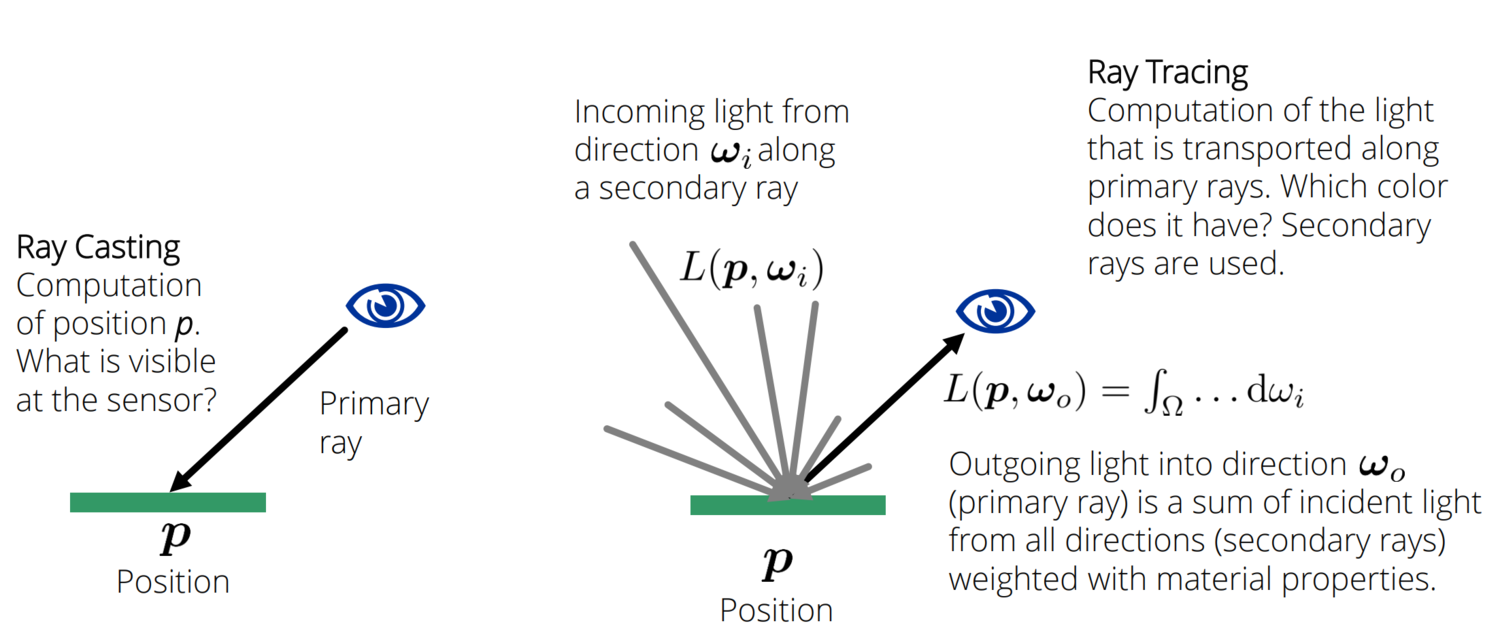
\includegraphics[width=.9\linewidth]{../graphics/casting-tracing.png}
    \caption{A demonstration of the difference between ray-casting and ray-tracing, together with an
    illustration of the recursive nature of the ray-casting algorithm. Taken
    from~\url{https://cg.informatik.uni-freiburg.de/course_notes/graphics_01_raycasting.pdf}.}\label{fig:casting_tracing}
\end{figure}

For rendering points with the classical approaches, surface splatting was proposed as a forward-projection approach that uses a z-buffer
algorithm for visibility resolution of points that are exchanged for oriented ellipses. Splatting can process point clouds
without additional acceleration data structures such as spatial hierarchies, which are
often required in ray-tracing approaches~\citep{PointRendering}. The initial article is mainly
a mathematical model and a CPU demonstrator that was later revisited by several papers that enhanced some of its
features and ported it to GPUs~\citep{Splatting2, Splatting3, Splatting4, Splatting5, Splatting6}.
Splatting can also be enriched with ray-tracing again to simulate more complex visual effects~\citep{SplattingTracing}.
Also, further GPU-related enhancements were proposed with better data structures suited for the usage~\citep{SequentialTrees}.\\

Another family of methods takes a vastly different approach than the classical rendering described
above---while traditional computer graphics
methods focus on modeling scenes from a physics perspective, simulating light transport and other effects,
machine learning can be used for modeling the distribution of real-world imagery. The models utilized for this task
are called generative models, successors of the work on \emph{Generative Adversarial Neural Networks}
(GANs)~\citep{GAN}, and can generate high-resolution images~\citep{ICLR, ICLR2} or videos~\citep{VPT, CDS}.
More specifically, the field of so-called neural rendering 
combines generative machine learning techniques with knowledge from classical computer
graphics. It is defined as \uv{deep image or video generation approaches that enable
explicit or implicit control of scene properties such as illumination, camera parameters, pose, geometry, appearance,
and semantic structure}~\citep{SOTARendering}. GANs produce \emph{random}, realistically-looking images that resemble
the training set~\citep{DGM} statistically. As the definition of neural rendering states, user controllability
is important---if used by an artist, outputs reflecting design ideas are preferred over some random imagery.
For applications in the neural rendering field, GANs thus needed to be extended by the conditioning of output
to enable guidance of the rendering process.

Further citing~\citet{SOTARendering}, neural rendering techniques can be classified along different axes:
\begin{itemize}
    \item \textbf{Control}. This axis distinguishes neural rendering approaches based on
    what properties from the definition are controllable and how they condition
    the network's output. A general solution enabling to control everything is an open
    research problem. Typically only a subset of controllable properties is approached
    in subproblems like novel view synthesis, relighting, or face and bodies animation.
    The conditioning can be performed by passing the scene parameters as input to some network
    layer or concatenating them to activations of an inner one, by tiling scene parameters over
    all pixels of an input image resulting in packed input volume, it can also employ
    an image-to-image transformation DNN that fuses \uv{guide image} into to the output one.
    Also, a more traditional approach uses scene parameters as an input to a graphical layer.
    \item \textbf{Computer Graphics Modules}. The separation along this axis is based on how much
    of the classical rendering pipeline is integrated into the specific method. The simplest way 
    to achieve that is to use a non-differentiable computer graphics (CG) component in the network
    architecture, which would present the render as an input to subsequent differentiable layers of a given architecture.
    When the module is at the beginning of the architecture, the task transforms into
    well-researched image-to-image translation. Fully differentiable CG modules also exist.
    \item \textbf{Explicit vs. Implicit Control}. Here, the criterion is based on a type of 
    control signal. Explicit control from a user perspective means manual editing capability
    of scene parameters in a semantically meaningful manner. By implicit control, a representative
    sample as input is meant. The difference also translates to training data as explicit control
    needs richer annotations, whereas implicit one performs well with less supervision.
    \item \textbf{Multi-modal Synthesis}. Not only from an art perspective, often it is beneficial to have
    multiple outputs from which a user can choose. Especially when only a subset of scene properties is
    controllable, within the rest, there lies an output space of possible results from which a given model
    can sample. This sampling capability adds complexity to the architecture, requiring some
    stochasticity or structured variance built-in, leading to GAN or variational auto-encoders (VAEs) variants.  % TODO clanek
    \item \textbf{Generality}. Does the rendering approach perform well over multiple
    scenes or objects without retraining the underlying model? Object-specific approaches
    still produce higher quality outputs at the cost of lengthy per-instance retraining. General models
    are still an open research area.
\end{itemize}

Methods spread across this classification landscape solve various subtasks of the neural rendering field.
Given the model this thesis utilizes, the novel view synthesis task is described next.\\

\emph{Novel view synthesis} generates a view of a
scene, represented by a fixed set of input images, from previously unexplored camera poses. Challenges tied to this task are inferring the scene's 3D
representation, given sparse observations in the form of images and deducing of occluded
or unseen areas of the scene. For the scene reconstruction, the aforementioned SfM is being utilized, followed by
MultiView Stereo (MVS)~\cite{MVS1, MVS2} or variational optimization~\cite{VarOpt}.

The classical computer vision approach towards novel view synthesis utilizes so-called image-based rendering (IBR)
methods~\citep{IBR1, IBR2, IBR3, IBR4} where views from new viewports are generated by warping input pixels into the
outputs using proxy geometry. These methods are sensitive to the scene database size as IBR may fail with insufficient number of source photos, resulting in ghosting-like artifacts and holes~\citep{SOTARendering}. These approaches
also do not handle multiple appearances well~\citep{NRIW}. Neural networks and
rendering alternative approaches have been proposed to mitigate these issues, such as~\citet{NR1, NR2, NRIW, InvSfM, FVS, SVS}.
These methods build on IBR and image-to-image translation using explicit scene models. Learned implicit
scene representation can be leveraged as well, see~\citet{NERF, NERF2, SceneRepr}.


\section{Neural Rerendering In the Wild}

According to the neural rendering techniques classification, the \emph{Neural Rerendering In the Wild} (NRIW) method~\citep{NRIW}
can be shortly described as a method explicitly controlling camera parameters, pose, and illumination, using
non-differentiable CG module preprocessing an input, producing multiple modalities, and being scene-specific.
More specifically, the authors tackle what they define as \emph{total scene capture} with a deep generative model that can
\begin{enumerate}
    \item perform novel view synthesis for a given scene,
    \item can capture and render various appearances of the scene, e.g., all
    weather and illumination conditions,
    \item and finally, it should understand the location and appearance of transient objects
    in the scene, such as people and vehicles, for reproducing or omitting them.
\end{enumerate}

Following~\citep{Bastien} in need of realistic point cloud renders, we utilize the model for
both indoor and outdoor rendering.

\uv{In the Wild} is related to unstructured photo collections from the internet NRIW can work with.
The method starts with building a proxy explicit 3D colored point cloud representation from a collection of
scene photos~$\{I_i\}$ by utilizing Structure-from-Motion (SfM) and MultiView Stereo (MVS) implemented by
COLMAP~\citep{schoenberger2016sfm, schoenberger2016mvs}. Authors prefer point clouds over generating a mesh
in a possible next step, even though meshes generate more complete renderings, as meshes \uv{also tend to contain pieces of misregistered floating geometry which can occlude large regions of the scene}. 

In the next stage, an aligned dataset of deferred-shading deep buffers $B_i$ is generated. Such a buffer,
in general, may contain per-pixel albedo, normal, depth, and any other derivative information. Authors use
a combination of rendered and real images~$\{I_i\}$, together with albedo and depth representations, all
depicting the same view. By the rendered image, a point splatting with a z-buffer with a radius of 1 pixel
render of the scene point cloud from a position $v_i$ recovered for the respective real image $I_i$ by SfM
is meant. Even though this may resemble an image-to-image translation paradigm, it is not the case as
such a model is uni-modal, not including appearance modeling. Image-to-image translation also fails to
understand transient objects in the scene.

The aligned dataset is used to train a multimodal image translation model. Its goal is to learn
a latent appearance vector~$z^a_i$ that captures variations in the output domain~$I_i$ that cannot be
inferred from the input domain~$B_i$. The method computes~$z^a_i$ as~$E^a(I_i, B_i)$, where~$E^a$ is
an appearance encoder of inputted~$I_i$ and~$B_i$ (the buffer is used for allowing the network to learn
more complex appearance models by correlating the lighting in the real image with scene geometry in the
corresponding buffer). Lastly, a rerendering network~$R$ produces a scene rendering conditioned
on both deep buffer~$B_i$ and the latent appearance vector~$z^a_i$. \cref{fig:nriw} presents a visual
overview of the process.

\begin{figure}
    \centering
    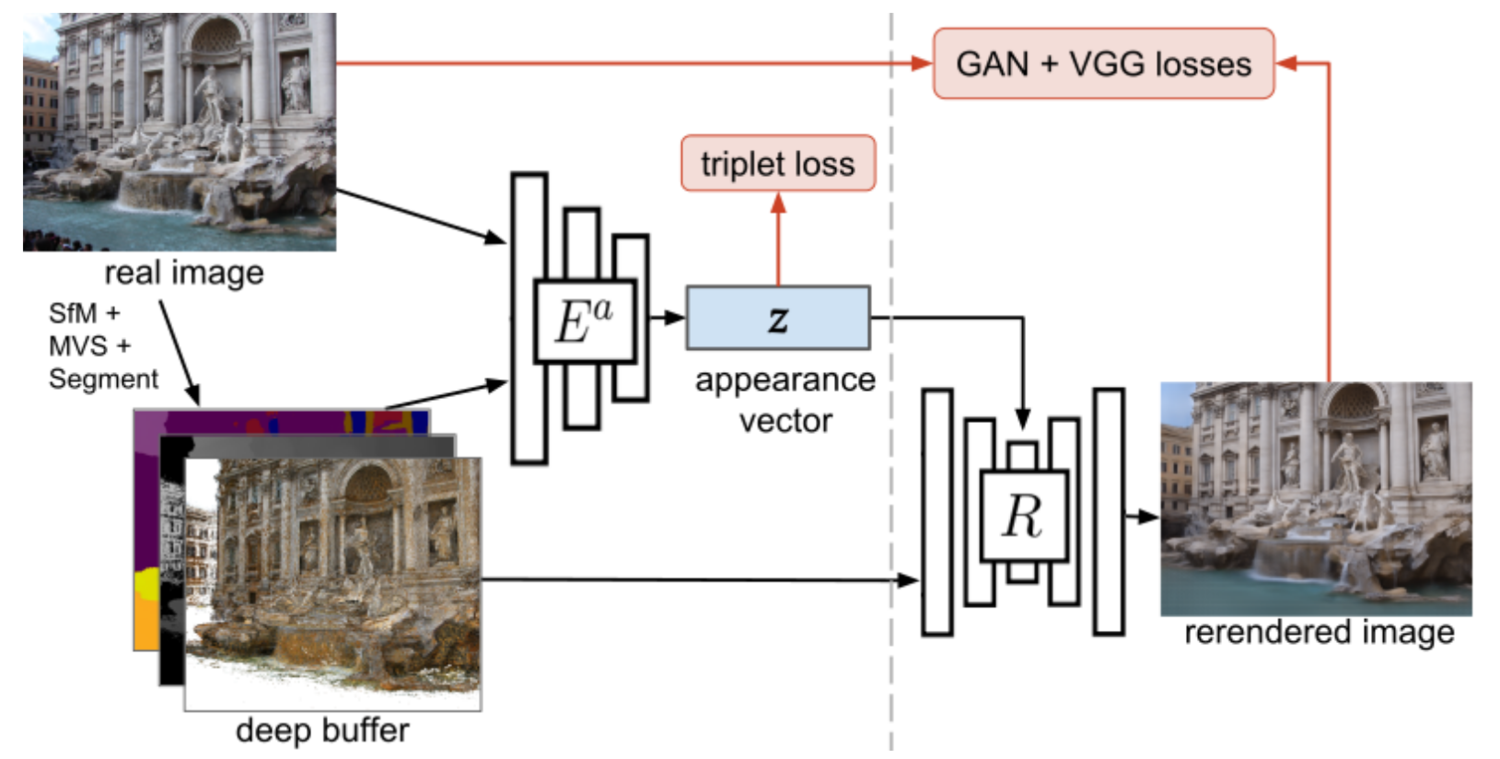
\includegraphics[width=.9\linewidth]{../graphics/nriw.png}
    \caption{Both neural networks are trained in a staged approach that pre-trains the appearance
    encoder~$E^a$ using a triplet loss, subsequently the rerenderer~$R$ is trained with standard
    reconstruction and GAN losses (right), and finally, fine-tuned together with~$E^a$.
    Taken from~\citet{NRIW}.}\label{fig:nriw}
\end{figure}

The training process works as follows---to stabilize the joint training of~$R$ and~$E^a$, and improve
the model expressiveness, pre-training the appearance encoder~$E^a$ on a proxy task is first performed.
In a staging manner, rendering network~$R$ is then trained using fixed~$E^a$ weights, allowing~$R$ to
find the correlations between output images and the embedding produced by the proxy task~$E^a$ training.
Finally, both networks are jointly fine-tuned.

The appearance pre-training works on a proxy task that optimizes
embeddings of the input images in the appearance latent space based on a suitable distance metric. Similar images under the metric should also have similar embeddings. The metric itself should ignore viewport as appearance is independent of it.
For that, authors use neural style-transfer triplet loss---for each image~$I_i$, sets of~$k$ closest and
farthest neighboring images with respect to the metric below are found. From those, one positive~$I_p$
and one negative~$I_n$ image is sampled, respectively. The loss then is:

$$\mathcal{L}(I_i, I_p, I_n) = \sum_j \mathrm{max}\left(\lVert g_i^j-g_p^j\rVert^2 - \lVert g_i^j-g_n^j\rVert^2 + \alpha, 0\right)\,,$$

where~$g_i^j$ is the Gram matrix of activations at the~$j$-th layer of a VGG network of image~$I_i$,
and~$\alpha$ is a separation margin.

Lastly, semantic conditioning performed by concatenating a semantic labeling~$S_i$ of
image~$I_i$ to the deep buffer~$B_i$ is used to account for transient objects. The authors argue that
it discourages the appearance encoder network from encoding variations caused by the location of
transient objects in the appearance latent space or associating such objects with specific viewports.

\section{Surface Splatting}

Surface splatting, presented by~\citet{SurfaceSplatting}, is an efficient technique for rendering high-quality
images of point clouds (point-sampled surfaces), supported by rigorous mathematical analysis around
resampling. In contrast to ray-tracing, it is a forward-projection approach that uses z-buffer to
resolve visibility. Also, it can avoid aliasing artifacts brought alongside discretizing otherwise
continuous space by a screen space formulation of the Elliptical Weighted Average (EWA) filter for
irregularly spaced point samples without global texture parameterization.

It can be seen as a resampling process in signal processing~\citep{PointRendering}, effectively the method
strives to reconstruct initially hole-free surfaces sampled in the form of a point cloud. To do so, the method
uses a combination of an object-space reconstruction filter and a screen-space filter for each point primitive.
The mathematical object-space reconstruction filter (\emph{footprint function}~$\rho_i(\mathbf{x})$ of a point~$\mathbf{x}$)
resembles typically an elliptical disk, a so-called splat whose position, orientation, and axes are usually
chosen to provide a good approximation to the underlying source geometry. After a perspective projection of all splats
to the screen space, the EWA filter mentioned above is used to avoid frequencies higher than the Nyquist frequency
of the pixel sampling grid, and all contributions from the overlapping splats are combined.

\SaveVerb{term}|GL_POINTS|
\begin{figure}
    \centering
    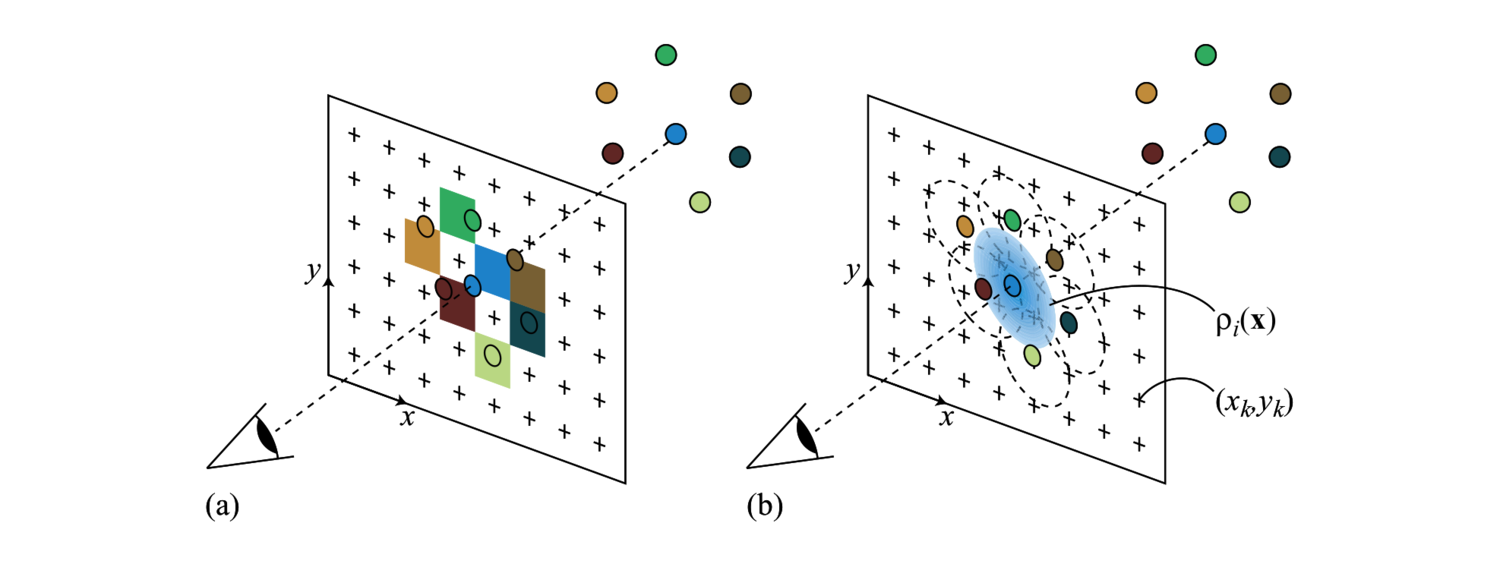
\includegraphics[width=.9\linewidth]{../graphics/splatting_principle.png}
    \caption{Point rendering by surface splatting compared to a naive approach that is used, for instance,
    by \protect\UseVerb{term} OpenGL primitive. (a) Naive forward projection and rendering of point samples
    assigning the projected point's color to the closest pixel in the screen space. (b) By splatting footprint
    functions, each pixel gets color decided upon a combination of contributions scree-space neighboring points.
    Taken from~\citet{PointRendering}.}\label{fig:splatting_principle}
\end{figure}

The basic idea of splatting compared to a naive approach is shown in~\cref{fig:splatting_principle}.
The naive method does not work generally as it leads to holes in reconstructed surfaces in the rendered image
if the surface is not sampled with sufficient frequency. Also, another disadvantage happens when more than
one point gets projected to the same closest pixel---then the rendering result depends on the order in
which the points are processed. Surface splatting alleviates the problems by distributing the color of
each projected point among more neighboring screen-space pixels with a suitable footprint function.
The desirable footprint function is usually smooth, decays quickly with increasing
distance from the projected center, and has local support as indicated by the ellipses in~\cref{fig:splatting_principle}.

For a single channel of a possible multiple-channel (taken independently) image, image function~$\phi(x, y)$
taking a pixel position and returning color could be defined according to previous thoughts as

\begin{equation}\label{eq:simple_splatting}
\phi(x, y) = \sum_i c_i\rho_i(x, y)\,,
\end{equation}
where the sum is carried over the indices of all points~$\{\mathbf{p}_i\}$ of the surface, $\rho_i$ are individual
footprint functions, and~$c_i$ are channel color values associated with a given point.

The definition~\cref{eq:simple_splatting} has an issue with reproducing surfaces with constant color and thus can
lead to visible artifacts. Also, footprint functions are truncated to finite support. Both leads to the below presented
normalized image function used by surface splatting

\begin{equation}\label{eq:normalized_splatting}
\phi(x, y) = \sum_i c_i\frac{\rho_i(x, y)}{\sum_k \rho_k(x, y)}\,.
\end{equation}
The image function defined by~\cref{eq:normalized_splatting} leads to a two-pass algorithm for
rendering~\cref{algo:splatting}. In the first pass, all points are iterated over and their splat
footprints~$\rho_i$ and channel values~$c_i$ are computed. The footprint functions are evaluated at each pixel, or
rasterized, and their contributions are accumulated in a buffer. At each pixel~$(x, y)$,
the buffer stores the sum of the weighted contributions from the right side of~\cref{eq:simple_splatting},
normalization factor sum from the denominator of~\cref{eq:normalized_splatting} and the depth for z-buffering.
In the second pass, all pixels are processed by normalization of the accumulated contributions by the accumulated
normalization factor.

\begin{algorithm}
	\caption{Pseudocode of the splatting algorithm.}\label{algo:splatting}
	\begin{algorithmic}[1]
		\Procedure{splat\_rendering}{p[], c[], w[], z[]}
			\For{all points i \textbf{in} p[]}
					\State rho\_i $\gets$ footprint(p\_i)
					\State c\_i $\gets$ shade(p\_i)
                        \State rasterize(rho\_i, c\_i, c[], w[], z[])
			\EndFor
			\For{all points [x, y]}
                        \State c[x, y] /= w[x, y]
			\EndFor
		\EndProcedure
	\end{algorithmic}
\end{algorithm}

How usable footprint functions are found and look is beyond the scope of this work as it requires
signal-processing theory, Gaussian functions, and the Nyquist theorem. We utilize
a GPU implementation by Sebastian Lipponer\footnotei{.}{\url{https://github.com/sebastianlipponer/surface_splatting}}

\section{Ray Marching with Signed Distance Fields}

This method is an example of a ray-casting approach, in which a finite series of steps along
a ray cast from a camera through a pixel is undertaken, until the ray hits an object or
the maximum number of permitted steps is exceeded. This very simple idea is fundamental in
computer graphics and dates back to works like~\citet{RayMarching, Hypertexture}. Building
on the idea, many effects, such as lights, shadows, and transparency, can be incorporated, to
name a few~\citep{RealTimeRendering}. This thesis implements a variant of the method using 
\emph{signed distance functions} (SDF).

In a given scene consisting of solid bodies, a \emph{signed distance function} is a simple scalar
function~$S(P)$ defined at every point~$P$ in a (2D or 3D) space, such that

\begin{equation}\label{eq:sdf_def}
\begin{array}{ll}
S(P) = 0 & \text{when it is on the surface of a body,}\\
S(P) > 0 & \text{when it is inside any body,}\\
S(P) < 0 & \text{when it is outside all bodies~\citep{SDF}.}
\end{array}
\end{equation}

A \emph{scene SDF} defines the scene implicitly. An \emph{object SDF} is the SDF of a scene containing
only that one object. Object SDFs can be computed analytically for simple shapes; see 
work of Inigo Quilez\footnotei{,}{\url{https://iquilezles.org/articles/distfunctions/}}
or tabulated in grids, octrees, or other spatial data structures. A scene SDF can then be constructed
by combining SDFs of objects in the scene. For simple analytically-describable shapes, an
insight into how such a scene can be built may be given through Constructive
Solid Geometry (CSG), a method of creating complex geometric shapes from simple ones via boolean
operations, see the left of~\cref{fig:rm}. This process has its mirror in combining SDFs; see code example in~\cref{code:sdfs}.
As an example, an SDF for the simplest 3D object, a sphere positioned at the origin and with a defined radius,
is \verb|SDF_sphere(vec3 pos) -> length(pos) - RADIUS|. In general, SDF does not need to be based on Euclidean distance
and may be exact or approximate. The only theoretical requirement is~\cref{eq:sdf_def} and from a practicality perspective,
evaluation of such a function should be reasonably quick.
The algorithm utilizing a scene SDF is outlined in~\cref{algo:marching}. The visual representation of
the simplest form of the algorithm proceeding along a ray is to be found in the right of~\cref{fig:rm}.

\begin{lstlisting}[language=Python,caption=Code example showing how SDFs of simpler object can be combined together to gradually build a scene SDF., label=code:sdfs]
def SDFintersect(obj1_SDF, obj2_SDF):
    return max(obj1_SDF, obj2_SDF)

def SDFunion(obj1_SDF, obj2_SDF):
    return min(obj1_SDF, obj2_SDF)

def SDFdifference(obj1_SDF, obj2_SDF):
    return max(obj1_SDF, -obj2_SDF)
\end{lstlisting}

\begin{figure}
	\centering
	\begin{subfigure}{.5\textwidth}
		\centering
		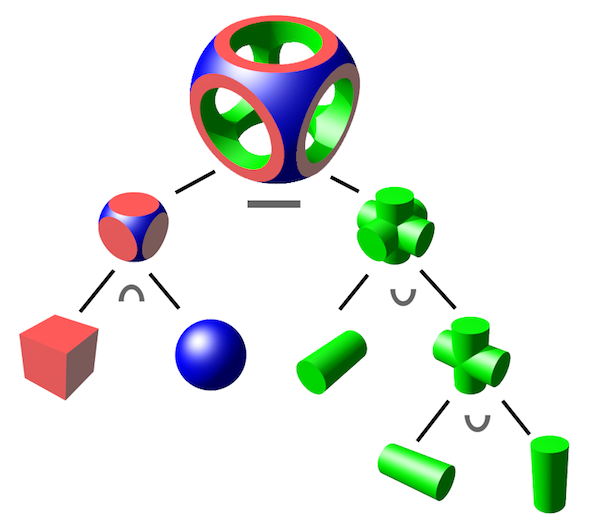
\includegraphics[width=.9\linewidth]{../graphics/csg.png}\label{fig:csg}
	\end{subfigure}%
	\begin{subfigure}{.5\textwidth}
		\centering
		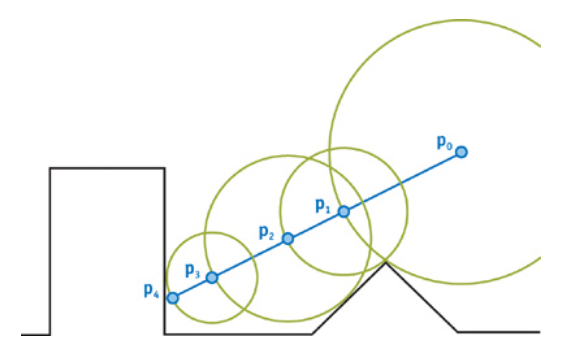
\includegraphics[width=.9\linewidth]{../graphics/marching.png} \label{fig:marching}
	\end{subfigure}
	\caption{Left: CSG is built upon three primitive operations: intersection ($\cap$),
        union ($\cup$), and difference ($-$).
        Taken from~\url{https://en.wikipedia.org/wiki/Constructive_solid_geometry}. Right: Demonstration
        of ray marching where at each step algorithm proceeds along given ray by a distance to the
        closest surface as it is a safe way how to find a hit, based on some threshold distance.
        Taken from~\url{https://jamie-wong.com/2016/07/15/ray-marching-signed-distance-functions/}.} \label{fig:rm}
\end{figure}

In this thesis, we utilize scene representation relying on translated sphere SDFs with radii precomputed beforehand
to be dependent on the distance to the closest neighbor for a given point primitive. Scene SDF for such a
scene would be then a minimum of all point SDFs in the scene (following again~\cref{code:sdfs}). This naive
declaration is not scalable to millions of points a scene produced by a LiDAR or SfM may contain, even though
only the simplest point primitives are used for the rendering process. To increase significantly rendering performance
with sufficient reality reproduction capabilities, we take advantage of a spatial 3D KD-tree~\citep{KDTree}
implemented in NVIDIA CUDA\footnote{\url{https://developer.nvidia.com/cuda-toolkit}} toolkit that can quickly
return the closest point for a given location. Since the exact sphere SDF contains its radius and KD-tree built
on top of the source point cloud returns the distance to the sphere center (point) itself, not the distance to the sphere's surface,
we take~$N$ closest points, instead of just one, compute exact SDF for those with their respective radii, and then take the point
at the minimal distance determined. The same KD-tree is pre-build once at the start of the rendering process and
is also used for radii computation instead of computing those exhaustively.

    
\begin{algorithm}
    \caption{Pseudocode of the ray marching with SDF.}\label{algo:marching}
    \begin{algorithmic}[1]
        \Procedure{ray\_march}{ray\_origin, ray\_direction}
            \State dist $\gets$ 0
            \For{i \textbf{in} range(MAX\_STEPS)}\Comment{Hyperparameter to stop traversal}
                \State current\_pos $\gets$ ray\_origin $+$ dist $*$ ray\_direction
                \State closest $\gets$ SDFscene(current\_pos)
                \If{closest.dist $<$ MIN\_HIT\_DIST}\Comment{Float comparison}
                    \State \textbf{return} closest.color
                \EndIf
                \If{dist $>$ MAX\_DIST}\Comment{No hit along the ray}
                    \State \textbf{return} BACKGROUND\_COLOR
                \EndIf
                \State dist $\gets$ dist $+$ closest.dist
            \EndFor
        \EndProcedure
    \end{algorithmic}
\end{algorithm}
